% Created by tikzDevice version 0.9 on 2016-03-14 23:38:45
% !TEX encoding = UTF-8 Unicode
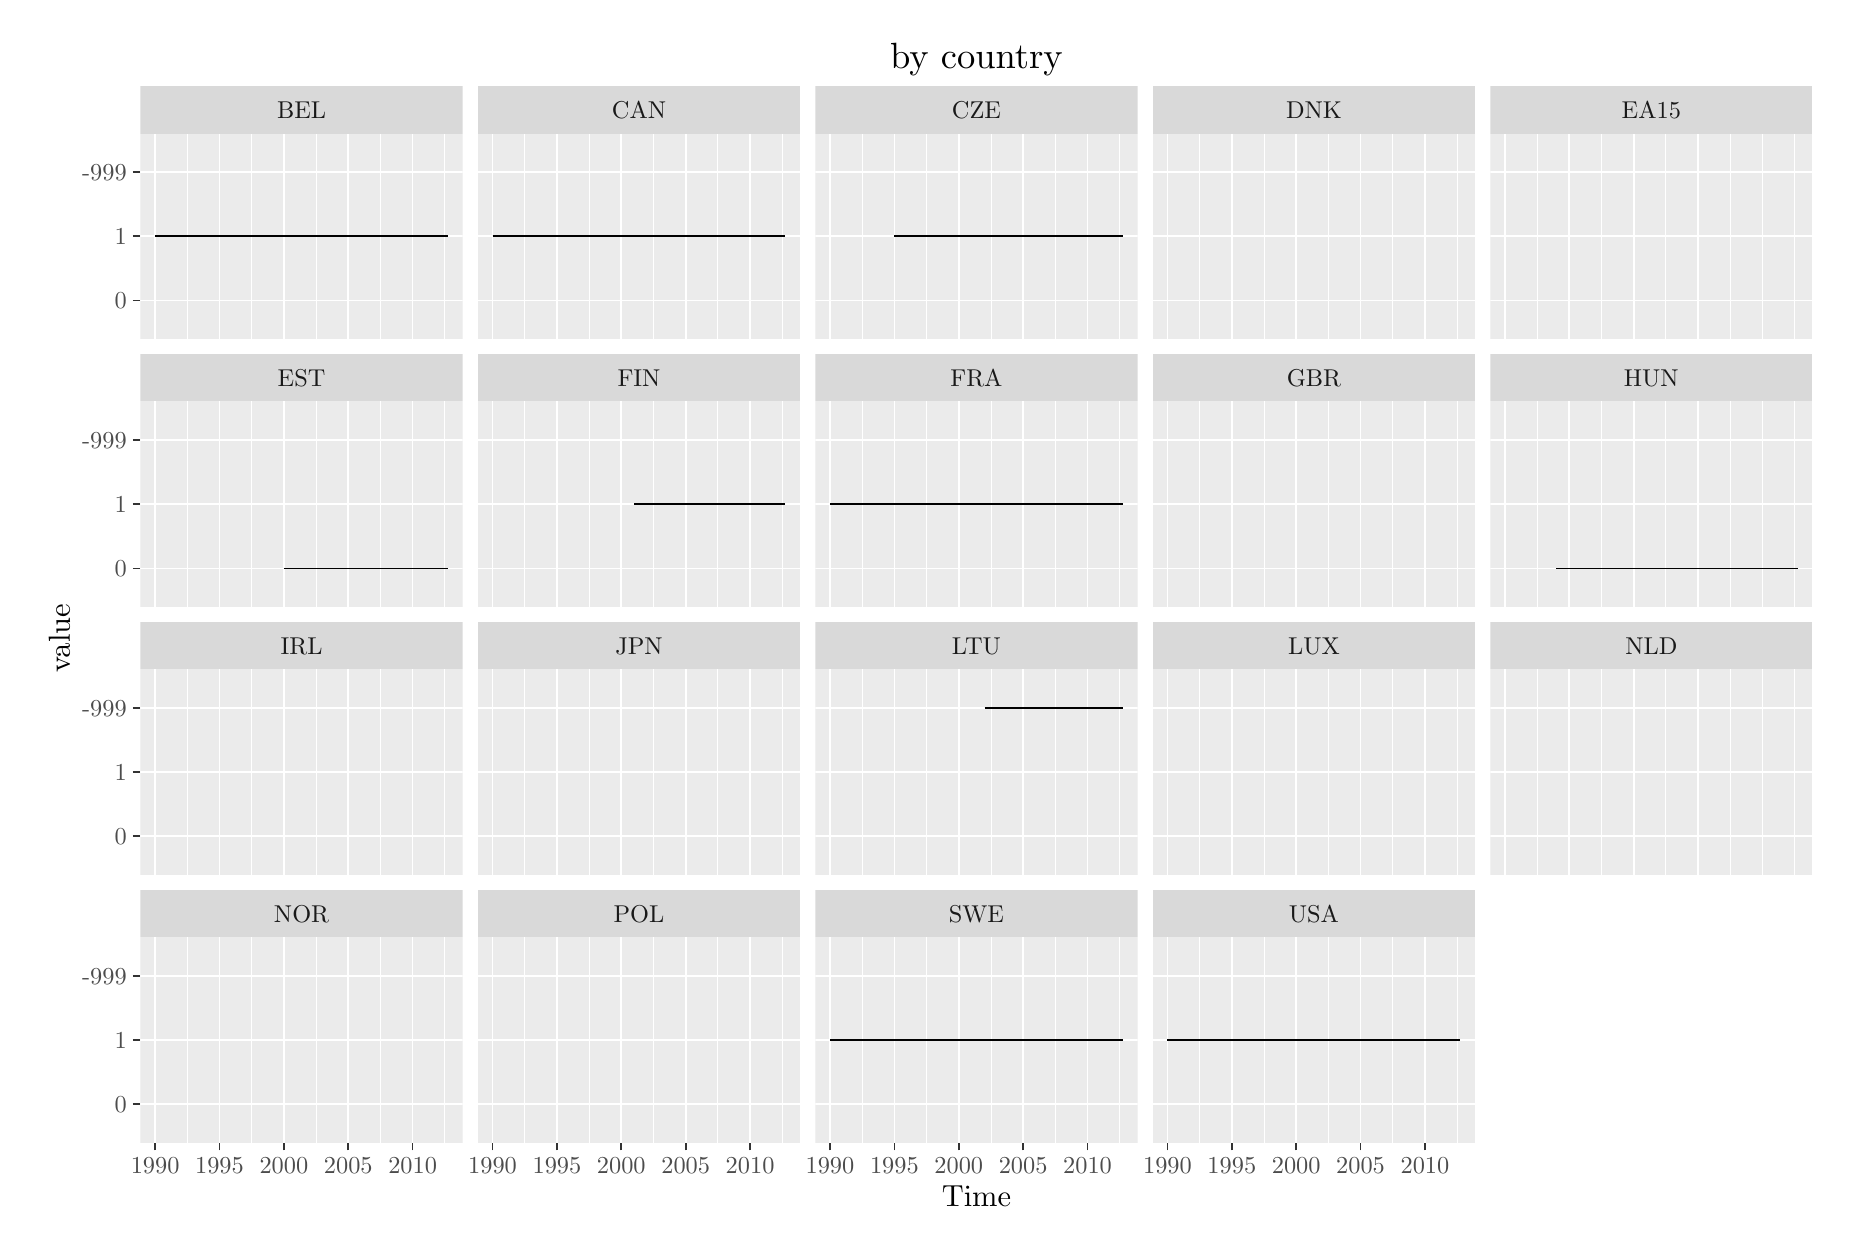
\begin{tikzpicture}[x=1pt,y=1pt]
\definecolor{fillColor}{RGB}{255,255,255}
\path[use as bounding box,fill=fillColor,fill opacity=0.00] (0,0) rectangle (650.43,433.62);
\begin{scope}
\path[clip] (  0.00,  0.00) rectangle (650.43,433.62);
\definecolor{drawColor}{RGB}{255,255,255}
\definecolor{fillColor}{RGB}{255,255,255}

\path[draw=drawColor,line width= 0.6pt,line join=round,line cap=round,fill=fillColor] (  0.00,  0.00) rectangle (650.43,433.62);
\end{scope}
\begin{scope}
\path[clip] ( 40.76,321.12) rectangle (157.19,395.37);
\definecolor{fillColor}{gray}{0.92}

\path[fill=fillColor] ( 40.76,321.12) rectangle (157.19,395.37);
\definecolor{drawColor}{RGB}{255,255,255}

\path[draw=drawColor,line width= 0.3pt,line join=round] ( 57.68,321.12) --
	( 57.68,395.37);

\path[draw=drawColor,line width= 0.3pt,line join=round] ( 80.94,321.12) --
	( 80.94,395.37);

\path[draw=drawColor,line width= 0.3pt,line join=round] (104.21,321.12) --
	(104.21,395.37);

\path[draw=drawColor,line width= 0.3pt,line join=round] (127.47,321.12) --
	(127.47,395.37);

\path[draw=drawColor,line width= 0.3pt,line join=round] (150.73,321.12) --
	(150.73,395.37);

\path[draw=drawColor,line width= 0.6pt,line join=round] ( 40.76,335.04) --
	(157.19,335.04);

\path[draw=drawColor,line width= 0.6pt,line join=round] ( 40.76,358.24) --
	(157.19,358.24);

\path[draw=drawColor,line width= 0.6pt,line join=round] ( 40.76,381.45) --
	(157.19,381.45);

\path[draw=drawColor,line width= 0.6pt,line join=round] ( 46.05,321.12) --
	( 46.05,395.37);

\path[draw=drawColor,line width= 0.6pt,line join=round] ( 69.31,321.12) --
	( 69.31,395.37);

\path[draw=drawColor,line width= 0.6pt,line join=round] ( 92.58,321.12) --
	( 92.58,395.37);

\path[draw=drawColor,line width= 0.6pt,line join=round] (115.84,321.12) --
	(115.84,395.37);

\path[draw=drawColor,line width= 0.6pt,line join=round] (139.10,321.12) --
	(139.10,395.37);
\definecolor{drawColor}{RGB}{0,0,0}

\path[draw=drawColor,line width= 0.6pt,line join=round] ( 46.05,358.24) --
	( 47.21,358.24) --
	( 48.37,358.24) --
	( 49.54,358.24) --
	( 50.70,358.24) --
	( 51.86,358.24) --
	( 53.03,358.24) --
	( 54.19,358.24) --
	( 55.35,358.24) --
	( 56.52,358.24) --
	( 57.68,358.24) --
	( 58.84,358.24) --
	( 60.01,358.24) --
	( 61.17,358.24) --
	( 62.33,358.24) --
	( 63.50,358.24) --
	( 64.66,358.24) --
	( 65.82,358.24) --
	( 66.99,358.24) --
	( 68.15,358.24) --
	( 69.31,358.24) --
	( 70.47,358.24) --
	( 71.64,358.24) --
	( 72.80,358.24) --
	( 73.96,358.24) --
	( 75.13,358.24) --
	( 76.29,358.24) --
	( 77.45,358.24) --
	( 78.62,358.24) --
	( 79.78,358.24) --
	( 80.94,358.24) --
	( 82.11,358.24) --
	( 83.27,358.24) --
	( 84.43,358.24) --
	( 85.60,358.24) --
	( 86.76,358.24) --
	( 87.92,358.24) --
	( 89.09,358.24) --
	( 90.25,358.24) --
	( 91.41,358.24) --
	( 92.58,358.24) --
	( 93.74,358.24) --
	( 94.90,358.24) --
	( 96.06,358.24) --
	( 97.23,358.24) --
	( 98.39,358.24) --
	( 99.55,358.24) --
	(100.72,358.24) --
	(101.88,358.24) --
	(103.04,358.24) --
	(104.21,358.24) --
	(105.37,358.24) --
	(106.53,358.24) --
	(107.70,358.24) --
	(108.86,358.24) --
	(110.02,358.24) --
	(111.19,358.24) --
	(112.35,358.24) --
	(113.51,358.24) --
	(114.68,358.24) --
	(115.84,358.24) --
	(117.00,358.24) --
	(118.17,358.24) --
	(119.33,358.24) --
	(120.49,358.24) --
	(121.66,358.24) --
	(122.82,358.24) --
	(123.98,358.24) --
	(125.14,358.24) --
	(126.31,358.24) --
	(127.47,358.24) --
	(128.63,358.24) --
	(129.80,358.24) --
	(130.96,358.24) --
	(132.12,358.24) --
	(133.29,358.24) --
	(134.45,358.24) --
	(135.61,358.24) --
	(136.78,358.24) --
	(137.94,358.24) --
	(139.10,358.24) --
	(140.27,358.24) --
	(141.43,358.24) --
	(142.59,358.24) --
	(143.76,358.24) --
	(144.92,358.24) --
	(146.08,358.24) --
	(147.25,358.24) --
	(148.41,358.24) --
	(149.57,358.24) --
	(150.73,358.24) --
	(151.90,358.24);
\end{scope}
\begin{scope}
\path[clip] (162.69,321.12) rectangle (279.13,395.37);
\definecolor{fillColor}{gray}{0.92}

\path[fill=fillColor] (162.69,321.12) rectangle (279.13,395.37);
\definecolor{drawColor}{RGB}{255,255,255}

\path[draw=drawColor,line width= 0.3pt,line join=round] (179.61,321.12) --
	(179.61,395.37);

\path[draw=drawColor,line width= 0.3pt,line join=round] (202.88,321.12) --
	(202.88,395.37);

\path[draw=drawColor,line width= 0.3pt,line join=round] (226.14,321.12) --
	(226.14,395.37);

\path[draw=drawColor,line width= 0.3pt,line join=round] (249.41,321.12) --
	(249.41,395.37);

\path[draw=drawColor,line width= 0.3pt,line join=round] (272.67,321.12) --
	(272.67,395.37);

\path[draw=drawColor,line width= 0.6pt,line join=round] (162.69,335.04) --
	(279.13,335.04);

\path[draw=drawColor,line width= 0.6pt,line join=round] (162.69,358.24) --
	(279.13,358.24);

\path[draw=drawColor,line width= 0.6pt,line join=round] (162.69,381.45) --
	(279.13,381.45);

\path[draw=drawColor,line width= 0.6pt,line join=round] (167.98,321.12) --
	(167.98,395.37);

\path[draw=drawColor,line width= 0.6pt,line join=round] (191.25,321.12) --
	(191.25,395.37);

\path[draw=drawColor,line width= 0.6pt,line join=round] (214.51,321.12) --
	(214.51,395.37);

\path[draw=drawColor,line width= 0.6pt,line join=round] (237.77,321.12) --
	(237.77,395.37);

\path[draw=drawColor,line width= 0.6pt,line join=round] (261.04,321.12) --
	(261.04,395.37);
\definecolor{drawColor}{RGB}{0,0,0}

\path[draw=drawColor,line width= 0.6pt,line join=round] (167.98,358.24) --
	(169.15,358.24) --
	(170.31,358.24) --
	(171.47,358.24) --
	(172.64,358.24) --
	(173.80,358.24) --
	(174.96,358.24) --
	(176.13,358.24) --
	(177.29,358.24) --
	(178.45,358.24) --
	(179.61,358.24) --
	(180.78,358.24) --
	(181.94,358.24) --
	(183.10,358.24) --
	(184.27,358.24) --
	(185.43,358.24) --
	(186.59,358.24) --
	(187.76,358.24) --
	(188.92,358.24) --
	(190.08,358.24) --
	(191.25,358.24) --
	(192.41,358.24) --
	(193.57,358.24) --
	(194.74,358.24) --
	(195.90,358.24) --
	(197.06,358.24) --
	(198.23,358.24) --
	(199.39,358.24) --
	(200.55,358.24) --
	(201.72,358.24) --
	(202.88,358.24) --
	(204.04,358.24) --
	(205.20,358.24) --
	(206.37,358.24) --
	(207.53,358.24) --
	(208.69,358.24) --
	(209.86,358.24) --
	(211.02,358.24) --
	(212.18,358.24) --
	(213.35,358.24) --
	(214.51,358.24) --
	(215.67,358.24) --
	(216.84,358.24) --
	(218.00,358.24) --
	(219.16,358.24) --
	(220.33,358.24) --
	(221.49,358.24) --
	(222.65,358.24) --
	(223.82,358.24) --
	(224.98,358.24) --
	(226.14,358.24) --
	(227.31,358.24) --
	(228.47,358.24) --
	(229.63,358.24) --
	(230.79,358.24) --
	(231.96,358.24) --
	(233.12,358.24) --
	(234.28,358.24) --
	(235.45,358.24) --
	(236.61,358.24) --
	(237.77,358.24) --
	(238.94,358.24) --
	(240.10,358.24) --
	(241.26,358.24) --
	(242.43,358.24) --
	(243.59,358.24) --
	(244.75,358.24) --
	(245.92,358.24) --
	(247.08,358.24) --
	(248.24,358.24) --
	(249.41,358.24) --
	(250.57,358.24) --
	(251.73,358.24) --
	(252.90,358.24) --
	(254.06,358.24) --
	(255.22,358.24) --
	(256.38,358.24) --
	(257.55,358.24) --
	(258.71,358.24) --
	(259.87,358.24) --
	(261.04,358.24) --
	(262.20,358.24) --
	(263.36,358.24) --
	(264.53,358.24) --
	(265.69,358.24) --
	(266.85,358.24) --
	(268.02,358.24) --
	(269.18,358.24) --
	(270.34,358.24) --
	(271.51,358.24) --
	(272.67,358.24) --
	(273.83,358.24);
\end{scope}
\begin{scope}
\path[clip] (284.63,321.12) rectangle (401.06,395.37);
\definecolor{fillColor}{gray}{0.92}

\path[fill=fillColor] (284.63,321.12) rectangle (401.06,395.37);
\definecolor{drawColor}{RGB}{255,255,255}

\path[draw=drawColor,line width= 0.3pt,line join=round] (301.55,321.12) --
	(301.55,395.37);

\path[draw=drawColor,line width= 0.3pt,line join=round] (324.81,321.12) --
	(324.81,395.37);

\path[draw=drawColor,line width= 0.3pt,line join=round] (348.08,321.12) --
	(348.08,395.37);

\path[draw=drawColor,line width= 0.3pt,line join=round] (371.34,321.12) --
	(371.34,395.37);

\path[draw=drawColor,line width= 0.3pt,line join=round] (394.60,321.12) --
	(394.60,395.37);

\path[draw=drawColor,line width= 0.6pt,line join=round] (284.63,335.04) --
	(401.06,335.04);

\path[draw=drawColor,line width= 0.6pt,line join=round] (284.63,358.24) --
	(401.06,358.24);

\path[draw=drawColor,line width= 0.6pt,line join=round] (284.63,381.45) --
	(401.06,381.45);

\path[draw=drawColor,line width= 0.6pt,line join=round] (289.92,321.12) --
	(289.92,395.37);

\path[draw=drawColor,line width= 0.6pt,line join=round] (313.18,321.12) --
	(313.18,395.37);

\path[draw=drawColor,line width= 0.6pt,line join=round] (336.45,321.12) --
	(336.45,395.37);

\path[draw=drawColor,line width= 0.6pt,line join=round] (359.71,321.12) --
	(359.71,395.37);

\path[draw=drawColor,line width= 0.6pt,line join=round] (382.97,321.12) --
	(382.97,395.37);
\definecolor{drawColor}{RGB}{0,0,0}

\path[draw=drawColor,line width= 0.6pt,line join=round] (313.18,358.24) --
	(314.34,358.24) --
	(315.51,358.24) --
	(316.67,358.24) --
	(317.83,358.24) --
	(319.00,358.24) --
	(320.16,358.24) --
	(321.32,358.24) --
	(322.49,358.24) --
	(323.65,358.24) --
	(324.81,358.24) --
	(325.98,358.24) --
	(327.14,358.24) --
	(328.30,358.24) --
	(329.47,358.24) --
	(330.63,358.24) --
	(331.79,358.24) --
	(332.96,358.24) --
	(334.12,358.24) --
	(335.28,358.24) --
	(336.45,358.24) --
	(337.61,358.24) --
	(338.77,358.24) --
	(339.93,358.24) --
	(341.10,358.24) --
	(342.26,358.24) --
	(343.42,358.24) --
	(344.59,358.24) --
	(345.75,358.24) --
	(346.91,358.24) --
	(348.08,358.24) --
	(349.24,358.24) --
	(350.40,358.24) --
	(351.57,358.24) --
	(352.73,358.24) --
	(353.89,358.24) --
	(355.06,358.24) --
	(356.22,358.24) --
	(357.38,358.24) --
	(358.55,358.24) --
	(359.71,358.24) --
	(360.87,358.24) --
	(362.04,358.24) --
	(363.20,358.24) --
	(364.36,358.24) --
	(365.52,358.24) --
	(366.69,358.24) --
	(367.85,358.24) --
	(369.01,358.24) --
	(370.18,358.24) --
	(371.34,358.24) --
	(372.50,358.24) --
	(373.67,358.24) --
	(374.83,358.24) --
	(375.99,358.24) --
	(377.16,358.24) --
	(378.32,358.24) --
	(379.48,358.24) --
	(380.65,358.24) --
	(381.81,358.24) --
	(382.97,358.24) --
	(384.14,358.24) --
	(385.30,358.24) --
	(386.46,358.24) --
	(387.63,358.24) --
	(388.79,358.24) --
	(389.95,358.24) --
	(391.11,358.24) --
	(392.28,358.24) --
	(393.44,358.24) --
	(394.60,358.24) --
	(395.77,358.24);
\end{scope}
\begin{scope}
\path[clip] (406.56,321.12) rectangle (523.00,395.37);
\definecolor{fillColor}{gray}{0.92}

\path[fill=fillColor] (406.56,321.12) rectangle (523.00,395.37);
\definecolor{drawColor}{RGB}{255,255,255}

\path[draw=drawColor,line width= 0.3pt,line join=round] (423.48,321.12) --
	(423.48,395.37);

\path[draw=drawColor,line width= 0.3pt,line join=round] (446.75,321.12) --
	(446.75,395.37);

\path[draw=drawColor,line width= 0.3pt,line join=round] (470.01,321.12) --
	(470.01,395.37);

\path[draw=drawColor,line width= 0.3pt,line join=round] (493.28,321.12) --
	(493.28,395.37);

\path[draw=drawColor,line width= 0.3pt,line join=round] (516.54,321.12) --
	(516.54,395.37);

\path[draw=drawColor,line width= 0.6pt,line join=round] (406.56,335.04) --
	(523.00,335.04);

\path[draw=drawColor,line width= 0.6pt,line join=round] (406.56,358.24) --
	(523.00,358.24);

\path[draw=drawColor,line width= 0.6pt,line join=round] (406.56,381.45) --
	(523.00,381.45);

\path[draw=drawColor,line width= 0.6pt,line join=round] (411.85,321.12) --
	(411.85,395.37);

\path[draw=drawColor,line width= 0.6pt,line join=round] (435.12,321.12) --
	(435.12,395.37);

\path[draw=drawColor,line width= 0.6pt,line join=round] (458.38,321.12) --
	(458.38,395.37);

\path[draw=drawColor,line width= 0.6pt,line join=round] (481.64,321.12) --
	(481.64,395.37);

\path[draw=drawColor,line width= 0.6pt,line join=round] (504.91,321.12) --
	(504.91,395.37);
\end{scope}
\begin{scope}
\path[clip] (528.50,321.12) rectangle (644.93,395.37);
\definecolor{fillColor}{gray}{0.92}

\path[fill=fillColor] (528.50,321.12) rectangle (644.93,395.37);
\definecolor{drawColor}{RGB}{255,255,255}

\path[draw=drawColor,line width= 0.3pt,line join=round] (545.42,321.12) --
	(545.42,395.37);

\path[draw=drawColor,line width= 0.3pt,line join=round] (568.68,321.12) --
	(568.68,395.37);

\path[draw=drawColor,line width= 0.3pt,line join=round] (591.95,321.12) --
	(591.95,395.37);

\path[draw=drawColor,line width= 0.3pt,line join=round] (615.21,321.12) --
	(615.21,395.37);

\path[draw=drawColor,line width= 0.3pt,line join=round] (638.47,321.12) --
	(638.47,395.37);

\path[draw=drawColor,line width= 0.6pt,line join=round] (528.50,335.04) --
	(644.93,335.04);

\path[draw=drawColor,line width= 0.6pt,line join=round] (528.50,358.24) --
	(644.93,358.24);

\path[draw=drawColor,line width= 0.6pt,line join=round] (528.50,381.45) --
	(644.93,381.45);

\path[draw=drawColor,line width= 0.6pt,line join=round] (533.79,321.12) --
	(533.79,395.37);

\path[draw=drawColor,line width= 0.6pt,line join=round] (557.05,321.12) --
	(557.05,395.37);

\path[draw=drawColor,line width= 0.6pt,line join=round] (580.32,321.12) --
	(580.32,395.37);

\path[draw=drawColor,line width= 0.6pt,line join=round] (603.58,321.12) --
	(603.58,395.37);

\path[draw=drawColor,line width= 0.6pt,line join=round] (626.84,321.12) --
	(626.84,395.37);
\end{scope}
\begin{scope}
\path[clip] ( 40.76,224.31) rectangle (157.19,298.56);
\definecolor{fillColor}{gray}{0.92}

\path[fill=fillColor] ( 40.76,224.31) rectangle (157.19,298.56);
\definecolor{drawColor}{RGB}{255,255,255}

\path[draw=drawColor,line width= 0.3pt,line join=round] ( 57.68,224.31) --
	( 57.68,298.56);

\path[draw=drawColor,line width= 0.3pt,line join=round] ( 80.94,224.31) --
	( 80.94,298.56);

\path[draw=drawColor,line width= 0.3pt,line join=round] (104.21,224.31) --
	(104.21,298.56);

\path[draw=drawColor,line width= 0.3pt,line join=round] (127.47,224.31) --
	(127.47,298.56);

\path[draw=drawColor,line width= 0.3pt,line join=round] (150.73,224.31) --
	(150.73,298.56);

\path[draw=drawColor,line width= 0.6pt,line join=round] ( 40.76,238.23) --
	(157.19,238.23);

\path[draw=drawColor,line width= 0.6pt,line join=round] ( 40.76,261.43) --
	(157.19,261.43);

\path[draw=drawColor,line width= 0.6pt,line join=round] ( 40.76,284.64) --
	(157.19,284.64);

\path[draw=drawColor,line width= 0.6pt,line join=round] ( 46.05,224.31) --
	( 46.05,298.56);

\path[draw=drawColor,line width= 0.6pt,line join=round] ( 69.31,224.31) --
	( 69.31,298.56);

\path[draw=drawColor,line width= 0.6pt,line join=round] ( 92.58,224.31) --
	( 92.58,298.56);

\path[draw=drawColor,line width= 0.6pt,line join=round] (115.84,224.31) --
	(115.84,298.56);

\path[draw=drawColor,line width= 0.6pt,line join=round] (139.10,224.31) --
	(139.10,298.56);
\definecolor{drawColor}{RGB}{0,0,0}

\path[draw=drawColor,line width= 0.6pt,line join=round] ( 92.58,238.23) --
	( 93.74,238.23) --
	( 94.90,238.23) --
	( 96.06,238.23) --
	( 97.23,238.23) --
	( 98.39,238.23) --
	( 99.55,238.23) --
	(100.72,238.23) --
	(101.88,238.23) --
	(103.04,238.23) --
	(104.21,238.23) --
	(105.37,238.23) --
	(106.53,238.23) --
	(107.70,238.23) --
	(108.86,238.23) --
	(110.02,238.23) --
	(111.19,238.23) --
	(112.35,238.23) --
	(113.51,238.23) --
	(114.68,238.23) --
	(115.84,238.23) --
	(117.00,238.23) --
	(118.17,238.23) --
	(119.33,238.23) --
	(120.49,238.23) --
	(121.66,238.23) --
	(122.82,238.23) --
	(123.98,238.23) --
	(125.14,238.23) --
	(126.31,238.23) --
	(127.47,238.23) --
	(128.63,238.23) --
	(129.80,238.23) --
	(130.96,238.23) --
	(132.12,238.23) --
	(133.29,238.23) --
	(134.45,238.23) --
	(135.61,238.23) --
	(136.78,238.23) --
	(137.94,238.23) --
	(139.10,238.23) --
	(140.27,238.23) --
	(141.43,238.23) --
	(142.59,238.23) --
	(143.76,238.23) --
	(144.92,238.23) --
	(146.08,238.23) --
	(147.25,238.23) --
	(148.41,238.23) --
	(149.57,238.23) --
	(150.73,238.23) --
	(151.90,238.23);
\end{scope}
\begin{scope}
\path[clip] (162.69,224.31) rectangle (279.13,298.56);
\definecolor{fillColor}{gray}{0.92}

\path[fill=fillColor] (162.69,224.31) rectangle (279.13,298.56);
\definecolor{drawColor}{RGB}{255,255,255}

\path[draw=drawColor,line width= 0.3pt,line join=round] (179.61,224.31) --
	(179.61,298.56);

\path[draw=drawColor,line width= 0.3pt,line join=round] (202.88,224.31) --
	(202.88,298.56);

\path[draw=drawColor,line width= 0.3pt,line join=round] (226.14,224.31) --
	(226.14,298.56);

\path[draw=drawColor,line width= 0.3pt,line join=round] (249.41,224.31) --
	(249.41,298.56);

\path[draw=drawColor,line width= 0.3pt,line join=round] (272.67,224.31) --
	(272.67,298.56);

\path[draw=drawColor,line width= 0.6pt,line join=round] (162.69,238.23) --
	(279.13,238.23);

\path[draw=drawColor,line width= 0.6pt,line join=round] (162.69,261.43) --
	(279.13,261.43);

\path[draw=drawColor,line width= 0.6pt,line join=round] (162.69,284.64) --
	(279.13,284.64);

\path[draw=drawColor,line width= 0.6pt,line join=round] (167.98,224.31) --
	(167.98,298.56);

\path[draw=drawColor,line width= 0.6pt,line join=round] (191.25,224.31) --
	(191.25,298.56);

\path[draw=drawColor,line width= 0.6pt,line join=round] (214.51,224.31) --
	(214.51,298.56);

\path[draw=drawColor,line width= 0.6pt,line join=round] (237.77,224.31) --
	(237.77,298.56);

\path[draw=drawColor,line width= 0.6pt,line join=round] (261.04,224.31) --
	(261.04,298.56);
\definecolor{drawColor}{RGB}{0,0,0}

\path[draw=drawColor,line width= 0.6pt,line join=round] (219.16,261.43) --
	(220.33,261.43) --
	(221.49,261.43) --
	(222.65,261.43) --
	(223.82,261.43) --
	(224.98,261.43) --
	(226.14,261.43) --
	(227.31,261.43) --
	(228.47,261.43) --
	(229.63,261.43) --
	(230.79,261.43) --
	(231.96,261.43) --
	(233.12,261.43) --
	(234.28,261.43) --
	(235.45,261.43) --
	(236.61,261.43) --
	(237.77,261.43) --
	(238.94,261.43) --
	(240.10,261.43) --
	(241.26,261.43) --
	(242.43,261.43) --
	(243.59,261.43) --
	(244.75,261.43) --
	(245.92,261.43) --
	(247.08,261.43) --
	(248.24,261.43) --
	(249.41,261.43) --
	(250.57,261.43) --
	(251.73,261.43) --
	(252.90,261.43) --
	(254.06,261.43) --
	(255.22,261.43) --
	(256.38,261.43) --
	(257.55,261.43) --
	(258.71,261.43) --
	(259.87,261.43) --
	(261.04,261.43) --
	(262.20,261.43) --
	(263.36,261.43) --
	(264.53,261.43) --
	(265.69,261.43) --
	(266.85,261.43) --
	(268.02,261.43) --
	(269.18,261.43) --
	(270.34,261.43) --
	(271.51,261.43) --
	(272.67,261.43) --
	(273.83,261.43);
\end{scope}
\begin{scope}
\path[clip] (284.63,224.31) rectangle (401.06,298.56);
\definecolor{fillColor}{gray}{0.92}

\path[fill=fillColor] (284.63,224.31) rectangle (401.06,298.56);
\definecolor{drawColor}{RGB}{255,255,255}

\path[draw=drawColor,line width= 0.3pt,line join=round] (301.55,224.31) --
	(301.55,298.56);

\path[draw=drawColor,line width= 0.3pt,line join=round] (324.81,224.31) --
	(324.81,298.56);

\path[draw=drawColor,line width= 0.3pt,line join=round] (348.08,224.31) --
	(348.08,298.56);

\path[draw=drawColor,line width= 0.3pt,line join=round] (371.34,224.31) --
	(371.34,298.56);

\path[draw=drawColor,line width= 0.3pt,line join=round] (394.60,224.31) --
	(394.60,298.56);

\path[draw=drawColor,line width= 0.6pt,line join=round] (284.63,238.23) --
	(401.06,238.23);

\path[draw=drawColor,line width= 0.6pt,line join=round] (284.63,261.43) --
	(401.06,261.43);

\path[draw=drawColor,line width= 0.6pt,line join=round] (284.63,284.64) --
	(401.06,284.64);

\path[draw=drawColor,line width= 0.6pt,line join=round] (289.92,224.31) --
	(289.92,298.56);

\path[draw=drawColor,line width= 0.6pt,line join=round] (313.18,224.31) --
	(313.18,298.56);

\path[draw=drawColor,line width= 0.6pt,line join=round] (336.45,224.31) --
	(336.45,298.56);

\path[draw=drawColor,line width= 0.6pt,line join=round] (359.71,224.31) --
	(359.71,298.56);

\path[draw=drawColor,line width= 0.6pt,line join=round] (382.97,224.31) --
	(382.97,298.56);
\definecolor{drawColor}{RGB}{0,0,0}

\path[draw=drawColor,line width= 0.6pt,line join=round] (289.92,261.43) --
	(291.08,261.43) --
	(292.24,261.43) --
	(293.41,261.43) --
	(294.57,261.43) --
	(295.73,261.43) --
	(296.90,261.43) --
	(298.06,261.43) --
	(299.22,261.43) --
	(300.39,261.43) --
	(301.55,261.43) --
	(302.71,261.43) --
	(303.88,261.43) --
	(305.04,261.43) --
	(306.20,261.43) --
	(307.37,261.43) --
	(308.53,261.43) --
	(309.69,261.43) --
	(310.86,261.43) --
	(312.02,261.43) --
	(313.18,261.43) --
	(314.34,261.43) --
	(315.51,261.43) --
	(316.67,261.43) --
	(317.83,261.43) --
	(319.00,261.43) --
	(320.16,261.43) --
	(321.32,261.43) --
	(322.49,261.43) --
	(323.65,261.43) --
	(324.81,261.43) --
	(325.98,261.43) --
	(327.14,261.43) --
	(328.30,261.43) --
	(329.47,261.43) --
	(330.63,261.43) --
	(331.79,261.43) --
	(332.96,261.43) --
	(334.12,261.43) --
	(335.28,261.43) --
	(336.45,261.43) --
	(337.61,261.43) --
	(338.77,261.43) --
	(339.93,261.43) --
	(341.10,261.43) --
	(342.26,261.43) --
	(343.42,261.43) --
	(344.59,261.43) --
	(345.75,261.43) --
	(346.91,261.43) --
	(348.08,261.43) --
	(349.24,261.43) --
	(350.40,261.43) --
	(351.57,261.43) --
	(352.73,261.43) --
	(353.89,261.43) --
	(355.06,261.43) --
	(356.22,261.43) --
	(357.38,261.43) --
	(358.55,261.43) --
	(359.71,261.43) --
	(360.87,261.43) --
	(362.04,261.43) --
	(363.20,261.43) --
	(364.36,261.43) --
	(365.52,261.43) --
	(366.69,261.43) --
	(367.85,261.43) --
	(369.01,261.43) --
	(370.18,261.43) --
	(371.34,261.43) --
	(372.50,261.43) --
	(373.67,261.43) --
	(374.83,261.43) --
	(375.99,261.43) --
	(377.16,261.43) --
	(378.32,261.43) --
	(379.48,261.43) --
	(380.65,261.43) --
	(381.81,261.43) --
	(382.97,261.43) --
	(384.14,261.43) --
	(385.30,261.43) --
	(386.46,261.43) --
	(387.63,261.43) --
	(388.79,261.43) --
	(389.95,261.43) --
	(391.11,261.43) --
	(392.28,261.43) --
	(393.44,261.43) --
	(394.60,261.43) --
	(395.77,261.43);
\end{scope}
\begin{scope}
\path[clip] (406.56,224.31) rectangle (523.00,298.56);
\definecolor{fillColor}{gray}{0.92}

\path[fill=fillColor] (406.56,224.31) rectangle (523.00,298.56);
\definecolor{drawColor}{RGB}{255,255,255}

\path[draw=drawColor,line width= 0.3pt,line join=round] (423.48,224.31) --
	(423.48,298.56);

\path[draw=drawColor,line width= 0.3pt,line join=round] (446.75,224.31) --
	(446.75,298.56);

\path[draw=drawColor,line width= 0.3pt,line join=round] (470.01,224.31) --
	(470.01,298.56);

\path[draw=drawColor,line width= 0.3pt,line join=round] (493.28,224.31) --
	(493.28,298.56);

\path[draw=drawColor,line width= 0.3pt,line join=round] (516.54,224.31) --
	(516.54,298.56);

\path[draw=drawColor,line width= 0.6pt,line join=round] (406.56,238.23) --
	(523.00,238.23);

\path[draw=drawColor,line width= 0.6pt,line join=round] (406.56,261.43) --
	(523.00,261.43);

\path[draw=drawColor,line width= 0.6pt,line join=round] (406.56,284.64) --
	(523.00,284.64);

\path[draw=drawColor,line width= 0.6pt,line join=round] (411.85,224.31) --
	(411.85,298.56);

\path[draw=drawColor,line width= 0.6pt,line join=round] (435.12,224.31) --
	(435.12,298.56);

\path[draw=drawColor,line width= 0.6pt,line join=round] (458.38,224.31) --
	(458.38,298.56);

\path[draw=drawColor,line width= 0.6pt,line join=round] (481.64,224.31) --
	(481.64,298.56);

\path[draw=drawColor,line width= 0.6pt,line join=round] (504.91,224.31) --
	(504.91,298.56);
\end{scope}
\begin{scope}
\path[clip] (528.50,224.31) rectangle (644.93,298.56);
\definecolor{fillColor}{gray}{0.92}

\path[fill=fillColor] (528.50,224.31) rectangle (644.93,298.56);
\definecolor{drawColor}{RGB}{255,255,255}

\path[draw=drawColor,line width= 0.3pt,line join=round] (545.42,224.31) --
	(545.42,298.56);

\path[draw=drawColor,line width= 0.3pt,line join=round] (568.68,224.31) --
	(568.68,298.56);

\path[draw=drawColor,line width= 0.3pt,line join=round] (591.95,224.31) --
	(591.95,298.56);

\path[draw=drawColor,line width= 0.3pt,line join=round] (615.21,224.31) --
	(615.21,298.56);

\path[draw=drawColor,line width= 0.3pt,line join=round] (638.47,224.31) --
	(638.47,298.56);

\path[draw=drawColor,line width= 0.6pt,line join=round] (528.50,238.23) --
	(644.93,238.23);

\path[draw=drawColor,line width= 0.6pt,line join=round] (528.50,261.43) --
	(644.93,261.43);

\path[draw=drawColor,line width= 0.6pt,line join=round] (528.50,284.64) --
	(644.93,284.64);

\path[draw=drawColor,line width= 0.6pt,line join=round] (533.79,224.31) --
	(533.79,298.56);

\path[draw=drawColor,line width= 0.6pt,line join=round] (557.05,224.31) --
	(557.05,298.56);

\path[draw=drawColor,line width= 0.6pt,line join=round] (580.32,224.31) --
	(580.32,298.56);

\path[draw=drawColor,line width= 0.6pt,line join=round] (603.58,224.31) --
	(603.58,298.56);

\path[draw=drawColor,line width= 0.6pt,line join=round] (626.84,224.31) --
	(626.84,298.56);
\definecolor{drawColor}{RGB}{0,0,0}

\path[draw=drawColor,line width= 0.6pt,line join=round] (552.40,238.23) --
	(553.56,238.23) --
	(554.72,238.23) --
	(555.89,238.23) --
	(557.05,238.23) --
	(558.21,238.23) --
	(559.38,238.23) --
	(560.54,238.23) --
	(561.70,238.23) --
	(562.87,238.23) --
	(564.03,238.23) --
	(565.19,238.23) --
	(566.36,238.23) --
	(567.52,238.23) --
	(568.68,238.23) --
	(569.85,238.23) --
	(571.01,238.23) --
	(572.17,238.23) --
	(573.34,238.23) --
	(574.50,238.23) --
	(575.66,238.23) --
	(576.83,238.23) --
	(577.99,238.23) --
	(579.15,238.23) --
	(580.32,238.23) --
	(581.48,238.23) --
	(582.64,238.23) --
	(583.80,238.23) --
	(584.97,238.23) --
	(586.13,238.23) --
	(587.29,238.23) --
	(588.46,238.23) --
	(589.62,238.23) --
	(590.78,238.23) --
	(591.95,238.23) --
	(593.11,238.23) --
	(594.27,238.23) --
	(595.44,238.23) --
	(596.60,238.23) --
	(597.76,238.23) --
	(598.93,238.23) --
	(600.09,238.23) --
	(601.25,238.23) --
	(602.42,238.23) --
	(603.58,238.23) --
	(604.74,238.23) --
	(605.91,238.23) --
	(607.07,238.23) --
	(608.23,238.23) --
	(609.39,238.23) --
	(610.56,238.23) --
	(611.72,238.23) --
	(612.88,238.23) --
	(614.05,238.23) --
	(615.21,238.23) --
	(616.37,238.23) --
	(617.54,238.23) --
	(618.70,238.23) --
	(619.86,238.23) --
	(621.03,238.23) --
	(622.19,238.23) --
	(623.35,238.23) --
	(624.52,238.23) --
	(625.68,238.23) --
	(626.84,238.23) --
	(628.01,238.23) --
	(629.17,238.23) --
	(630.33,238.23) --
	(631.50,238.23) --
	(632.66,238.23) --
	(633.82,238.23) --
	(634.98,238.23) --
	(636.15,238.23) --
	(637.31,238.23) --
	(638.47,238.23) --
	(639.64,238.23);
\end{scope}
\begin{scope}
\path[clip] ( 40.76,127.50) rectangle (157.19,201.75);
\definecolor{fillColor}{gray}{0.92}

\path[fill=fillColor] ( 40.76,127.50) rectangle (157.19,201.75);
\definecolor{drawColor}{RGB}{255,255,255}

\path[draw=drawColor,line width= 0.3pt,line join=round] ( 57.68,127.50) --
	( 57.68,201.75);

\path[draw=drawColor,line width= 0.3pt,line join=round] ( 80.94,127.50) --
	( 80.94,201.75);

\path[draw=drawColor,line width= 0.3pt,line join=round] (104.21,127.50) --
	(104.21,201.75);

\path[draw=drawColor,line width= 0.3pt,line join=round] (127.47,127.50) --
	(127.47,201.75);

\path[draw=drawColor,line width= 0.3pt,line join=round] (150.73,127.50) --
	(150.73,201.75);

\path[draw=drawColor,line width= 0.6pt,line join=round] ( 40.76,141.42) --
	(157.19,141.42);

\path[draw=drawColor,line width= 0.6pt,line join=round] ( 40.76,164.62) --
	(157.19,164.62);

\path[draw=drawColor,line width= 0.6pt,line join=round] ( 40.76,187.83) --
	(157.19,187.83);

\path[draw=drawColor,line width= 0.6pt,line join=round] ( 46.05,127.50) --
	( 46.05,201.75);

\path[draw=drawColor,line width= 0.6pt,line join=round] ( 69.31,127.50) --
	( 69.31,201.75);

\path[draw=drawColor,line width= 0.6pt,line join=round] ( 92.58,127.50) --
	( 92.58,201.75);

\path[draw=drawColor,line width= 0.6pt,line join=round] (115.84,127.50) --
	(115.84,201.75);

\path[draw=drawColor,line width= 0.6pt,line join=round] (139.10,127.50) --
	(139.10,201.75);
\end{scope}
\begin{scope}
\path[clip] (162.69,127.50) rectangle (279.13,201.75);
\definecolor{fillColor}{gray}{0.92}

\path[fill=fillColor] (162.69,127.50) rectangle (279.13,201.75);
\definecolor{drawColor}{RGB}{255,255,255}

\path[draw=drawColor,line width= 0.3pt,line join=round] (179.61,127.50) --
	(179.61,201.75);

\path[draw=drawColor,line width= 0.3pt,line join=round] (202.88,127.50) --
	(202.88,201.75);

\path[draw=drawColor,line width= 0.3pt,line join=round] (226.14,127.50) --
	(226.14,201.75);

\path[draw=drawColor,line width= 0.3pt,line join=round] (249.41,127.50) --
	(249.41,201.75);

\path[draw=drawColor,line width= 0.3pt,line join=round] (272.67,127.50) --
	(272.67,201.75);

\path[draw=drawColor,line width= 0.6pt,line join=round] (162.69,141.42) --
	(279.13,141.42);

\path[draw=drawColor,line width= 0.6pt,line join=round] (162.69,164.62) --
	(279.13,164.62);

\path[draw=drawColor,line width= 0.6pt,line join=round] (162.69,187.83) --
	(279.13,187.83);

\path[draw=drawColor,line width= 0.6pt,line join=round] (167.98,127.50) --
	(167.98,201.75);

\path[draw=drawColor,line width= 0.6pt,line join=round] (191.25,127.50) --
	(191.25,201.75);

\path[draw=drawColor,line width= 0.6pt,line join=round] (214.51,127.50) --
	(214.51,201.75);

\path[draw=drawColor,line width= 0.6pt,line join=round] (237.77,127.50) --
	(237.77,201.75);

\path[draw=drawColor,line width= 0.6pt,line join=round] (261.04,127.50) --
	(261.04,201.75);
\end{scope}
\begin{scope}
\path[clip] (284.63,127.50) rectangle (401.06,201.75);
\definecolor{fillColor}{gray}{0.92}

\path[fill=fillColor] (284.63,127.50) rectangle (401.06,201.75);
\definecolor{drawColor}{RGB}{255,255,255}

\path[draw=drawColor,line width= 0.3pt,line join=round] (301.55,127.50) --
	(301.55,201.75);

\path[draw=drawColor,line width= 0.3pt,line join=round] (324.81,127.50) --
	(324.81,201.75);

\path[draw=drawColor,line width= 0.3pt,line join=round] (348.08,127.50) --
	(348.08,201.75);

\path[draw=drawColor,line width= 0.3pt,line join=round] (371.34,127.50) --
	(371.34,201.75);

\path[draw=drawColor,line width= 0.3pt,line join=round] (394.60,127.50) --
	(394.60,201.75);

\path[draw=drawColor,line width= 0.6pt,line join=round] (284.63,141.42) --
	(401.06,141.42);

\path[draw=drawColor,line width= 0.6pt,line join=round] (284.63,164.62) --
	(401.06,164.62);

\path[draw=drawColor,line width= 0.6pt,line join=round] (284.63,187.83) --
	(401.06,187.83);

\path[draw=drawColor,line width= 0.6pt,line join=round] (289.92,127.50) --
	(289.92,201.75);

\path[draw=drawColor,line width= 0.6pt,line join=round] (313.18,127.50) --
	(313.18,201.75);

\path[draw=drawColor,line width= 0.6pt,line join=round] (336.45,127.50) --
	(336.45,201.75);

\path[draw=drawColor,line width= 0.6pt,line join=round] (359.71,127.50) --
	(359.71,201.75);

\path[draw=drawColor,line width= 0.6pt,line join=round] (382.97,127.50) --
	(382.97,201.75);
\definecolor{drawColor}{RGB}{0,0,0}

\path[draw=drawColor,line width= 0.6pt,line join=round] (345.75,187.83) --
	(346.91,187.83) --
	(348.08,187.83) --
	(349.24,187.83) --
	(350.40,187.83) --
	(351.57,187.83) --
	(352.73,187.83) --
	(353.89,187.83) --
	(355.06,187.83) --
	(356.22,187.83) --
	(357.38,187.83) --
	(358.55,187.83) --
	(359.71,187.83) --
	(360.87,187.83) --
	(362.04,187.83) --
	(363.20,187.83) --
	(364.36,187.83) --
	(365.52,187.83) --
	(366.69,187.83) --
	(367.85,187.83) --
	(369.01,187.83) --
	(370.18,187.83) --
	(371.34,187.83) --
	(372.50,187.83) --
	(373.67,187.83) --
	(374.83,187.83) --
	(375.99,187.83) --
	(377.16,187.83) --
	(378.32,187.83) --
	(379.48,187.83) --
	(380.65,187.83) --
	(381.81,187.83) --
	(382.97,187.83) --
	(384.14,187.83) --
	(385.30,187.83) --
	(386.46,187.83) --
	(387.63,187.83) --
	(388.79,187.83) --
	(389.95,187.83) --
	(391.11,187.83) --
	(392.28,187.83) --
	(393.44,187.83) --
	(394.60,187.83) --
	(395.77,187.83);
\end{scope}
\begin{scope}
\path[clip] (406.56,127.50) rectangle (523.00,201.75);
\definecolor{fillColor}{gray}{0.92}

\path[fill=fillColor] (406.56,127.50) rectangle (523.00,201.75);
\definecolor{drawColor}{RGB}{255,255,255}

\path[draw=drawColor,line width= 0.3pt,line join=round] (423.48,127.50) --
	(423.48,201.75);

\path[draw=drawColor,line width= 0.3pt,line join=round] (446.75,127.50) --
	(446.75,201.75);

\path[draw=drawColor,line width= 0.3pt,line join=round] (470.01,127.50) --
	(470.01,201.75);

\path[draw=drawColor,line width= 0.3pt,line join=round] (493.28,127.50) --
	(493.28,201.75);

\path[draw=drawColor,line width= 0.3pt,line join=round] (516.54,127.50) --
	(516.54,201.75);

\path[draw=drawColor,line width= 0.6pt,line join=round] (406.56,141.42) --
	(523.00,141.42);

\path[draw=drawColor,line width= 0.6pt,line join=round] (406.56,164.62) --
	(523.00,164.62);

\path[draw=drawColor,line width= 0.6pt,line join=round] (406.56,187.83) --
	(523.00,187.83);

\path[draw=drawColor,line width= 0.6pt,line join=round] (411.85,127.50) --
	(411.85,201.75);

\path[draw=drawColor,line width= 0.6pt,line join=round] (435.12,127.50) --
	(435.12,201.75);

\path[draw=drawColor,line width= 0.6pt,line join=round] (458.38,127.50) --
	(458.38,201.75);

\path[draw=drawColor,line width= 0.6pt,line join=round] (481.64,127.50) --
	(481.64,201.75);

\path[draw=drawColor,line width= 0.6pt,line join=round] (504.91,127.50) --
	(504.91,201.75);
\end{scope}
\begin{scope}
\path[clip] (528.50,127.50) rectangle (644.93,201.75);
\definecolor{fillColor}{gray}{0.92}

\path[fill=fillColor] (528.50,127.50) rectangle (644.93,201.75);
\definecolor{drawColor}{RGB}{255,255,255}

\path[draw=drawColor,line width= 0.3pt,line join=round] (545.42,127.50) --
	(545.42,201.75);

\path[draw=drawColor,line width= 0.3pt,line join=round] (568.68,127.50) --
	(568.68,201.75);

\path[draw=drawColor,line width= 0.3pt,line join=round] (591.95,127.50) --
	(591.95,201.75);

\path[draw=drawColor,line width= 0.3pt,line join=round] (615.21,127.50) --
	(615.21,201.75);

\path[draw=drawColor,line width= 0.3pt,line join=round] (638.47,127.50) --
	(638.47,201.75);

\path[draw=drawColor,line width= 0.6pt,line join=round] (528.50,141.42) --
	(644.93,141.42);

\path[draw=drawColor,line width= 0.6pt,line join=round] (528.50,164.62) --
	(644.93,164.62);

\path[draw=drawColor,line width= 0.6pt,line join=round] (528.50,187.83) --
	(644.93,187.83);

\path[draw=drawColor,line width= 0.6pt,line join=round] (533.79,127.50) --
	(533.79,201.75);

\path[draw=drawColor,line width= 0.6pt,line join=round] (557.05,127.50) --
	(557.05,201.75);

\path[draw=drawColor,line width= 0.6pt,line join=round] (580.32,127.50) --
	(580.32,201.75);

\path[draw=drawColor,line width= 0.6pt,line join=round] (603.58,127.50) --
	(603.58,201.75);

\path[draw=drawColor,line width= 0.6pt,line join=round] (626.84,127.50) --
	(626.84,201.75);
\end{scope}
\begin{scope}
\path[clip] ( 40.76, 30.69) rectangle (157.19,104.94);
\definecolor{fillColor}{gray}{0.92}

\path[fill=fillColor] ( 40.76, 30.69) rectangle (157.19,104.94);
\definecolor{drawColor}{RGB}{255,255,255}

\path[draw=drawColor,line width= 0.3pt,line join=round] ( 57.68, 30.69) --
	( 57.68,104.94);

\path[draw=drawColor,line width= 0.3pt,line join=round] ( 80.94, 30.69) --
	( 80.94,104.94);

\path[draw=drawColor,line width= 0.3pt,line join=round] (104.21, 30.69) --
	(104.21,104.94);

\path[draw=drawColor,line width= 0.3pt,line join=round] (127.47, 30.69) --
	(127.47,104.94);

\path[draw=drawColor,line width= 0.3pt,line join=round] (150.73, 30.69) --
	(150.73,104.94);

\path[draw=drawColor,line width= 0.6pt,line join=round] ( 40.76, 44.61) --
	(157.19, 44.61);

\path[draw=drawColor,line width= 0.6pt,line join=round] ( 40.76, 67.81) --
	(157.19, 67.81);

\path[draw=drawColor,line width= 0.6pt,line join=round] ( 40.76, 91.01) --
	(157.19, 91.01);

\path[draw=drawColor,line width= 0.6pt,line join=round] ( 46.05, 30.69) --
	( 46.05,104.94);

\path[draw=drawColor,line width= 0.6pt,line join=round] ( 69.31, 30.69) --
	( 69.31,104.94);

\path[draw=drawColor,line width= 0.6pt,line join=round] ( 92.58, 30.69) --
	( 92.58,104.94);

\path[draw=drawColor,line width= 0.6pt,line join=round] (115.84, 30.69) --
	(115.84,104.94);

\path[draw=drawColor,line width= 0.6pt,line join=round] (139.10, 30.69) --
	(139.10,104.94);
\end{scope}
\begin{scope}
\path[clip] (162.69, 30.69) rectangle (279.13,104.94);
\definecolor{fillColor}{gray}{0.92}

\path[fill=fillColor] (162.69, 30.69) rectangle (279.13,104.94);
\definecolor{drawColor}{RGB}{255,255,255}

\path[draw=drawColor,line width= 0.3pt,line join=round] (179.61, 30.69) --
	(179.61,104.94);

\path[draw=drawColor,line width= 0.3pt,line join=round] (202.88, 30.69) --
	(202.88,104.94);

\path[draw=drawColor,line width= 0.3pt,line join=round] (226.14, 30.69) --
	(226.14,104.94);

\path[draw=drawColor,line width= 0.3pt,line join=round] (249.41, 30.69) --
	(249.41,104.94);

\path[draw=drawColor,line width= 0.3pt,line join=round] (272.67, 30.69) --
	(272.67,104.94);

\path[draw=drawColor,line width= 0.6pt,line join=round] (162.69, 44.61) --
	(279.13, 44.61);

\path[draw=drawColor,line width= 0.6pt,line join=round] (162.69, 67.81) --
	(279.13, 67.81);

\path[draw=drawColor,line width= 0.6pt,line join=round] (162.69, 91.01) --
	(279.13, 91.01);

\path[draw=drawColor,line width= 0.6pt,line join=round] (167.98, 30.69) --
	(167.98,104.94);

\path[draw=drawColor,line width= 0.6pt,line join=round] (191.25, 30.69) --
	(191.25,104.94);

\path[draw=drawColor,line width= 0.6pt,line join=round] (214.51, 30.69) --
	(214.51,104.94);

\path[draw=drawColor,line width= 0.6pt,line join=round] (237.77, 30.69) --
	(237.77,104.94);

\path[draw=drawColor,line width= 0.6pt,line join=round] (261.04, 30.69) --
	(261.04,104.94);
\end{scope}
\begin{scope}
\path[clip] (284.63, 30.69) rectangle (401.06,104.94);
\definecolor{fillColor}{gray}{0.92}

\path[fill=fillColor] (284.63, 30.69) rectangle (401.06,104.94);
\definecolor{drawColor}{RGB}{255,255,255}

\path[draw=drawColor,line width= 0.3pt,line join=round] (301.55, 30.69) --
	(301.55,104.94);

\path[draw=drawColor,line width= 0.3pt,line join=round] (324.81, 30.69) --
	(324.81,104.94);

\path[draw=drawColor,line width= 0.3pt,line join=round] (348.08, 30.69) --
	(348.08,104.94);

\path[draw=drawColor,line width= 0.3pt,line join=round] (371.34, 30.69) --
	(371.34,104.94);

\path[draw=drawColor,line width= 0.3pt,line join=round] (394.60, 30.69) --
	(394.60,104.94);

\path[draw=drawColor,line width= 0.6pt,line join=round] (284.63, 44.61) --
	(401.06, 44.61);

\path[draw=drawColor,line width= 0.6pt,line join=round] (284.63, 67.81) --
	(401.06, 67.81);

\path[draw=drawColor,line width= 0.6pt,line join=round] (284.63, 91.01) --
	(401.06, 91.01);

\path[draw=drawColor,line width= 0.6pt,line join=round] (289.92, 30.69) --
	(289.92,104.94);

\path[draw=drawColor,line width= 0.6pt,line join=round] (313.18, 30.69) --
	(313.18,104.94);

\path[draw=drawColor,line width= 0.6pt,line join=round] (336.45, 30.69) --
	(336.45,104.94);

\path[draw=drawColor,line width= 0.6pt,line join=round] (359.71, 30.69) --
	(359.71,104.94);

\path[draw=drawColor,line width= 0.6pt,line join=round] (382.97, 30.69) --
	(382.97,104.94);
\definecolor{drawColor}{RGB}{0,0,0}

\path[draw=drawColor,line width= 0.6pt,line join=round] (289.92, 67.81) --
	(291.08, 67.81) --
	(292.24, 67.81) --
	(293.41, 67.81) --
	(294.57, 67.81) --
	(295.73, 67.81) --
	(296.90, 67.81) --
	(298.06, 67.81) --
	(299.22, 67.81) --
	(300.39, 67.81) --
	(301.55, 67.81) --
	(302.71, 67.81) --
	(303.88, 67.81) --
	(305.04, 67.81) --
	(306.20, 67.81) --
	(307.37, 67.81) --
	(308.53, 67.81) --
	(309.69, 67.81) --
	(310.86, 67.81) --
	(312.02, 67.81) --
	(313.18, 67.81) --
	(314.34, 67.81) --
	(315.51, 67.81) --
	(316.67, 67.81) --
	(317.83, 67.81) --
	(319.00, 67.81) --
	(320.16, 67.81) --
	(321.32, 67.81) --
	(322.49, 67.81) --
	(323.65, 67.81) --
	(324.81, 67.81) --
	(325.98, 67.81) --
	(327.14, 67.81) --
	(328.30, 67.81) --
	(329.47, 67.81) --
	(330.63, 67.81) --
	(331.79, 67.81) --
	(332.96, 67.81) --
	(334.12, 67.81) --
	(335.28, 67.81) --
	(336.45, 67.81) --
	(337.61, 67.81) --
	(338.77, 67.81) --
	(339.93, 67.81) --
	(341.10, 67.81) --
	(342.26, 67.81) --
	(343.42, 67.81) --
	(344.59, 67.81) --
	(345.75, 67.81) --
	(346.91, 67.81) --
	(348.08, 67.81) --
	(349.24, 67.81) --
	(350.40, 67.81) --
	(351.57, 67.81) --
	(352.73, 67.81) --
	(353.89, 67.81) --
	(355.06, 67.81) --
	(356.22, 67.81) --
	(357.38, 67.81) --
	(358.55, 67.81) --
	(359.71, 67.81) --
	(360.87, 67.81) --
	(362.04, 67.81) --
	(363.20, 67.81) --
	(364.36, 67.81) --
	(365.52, 67.81) --
	(366.69, 67.81) --
	(367.85, 67.81) --
	(369.01, 67.81) --
	(370.18, 67.81) --
	(371.34, 67.81) --
	(372.50, 67.81) --
	(373.67, 67.81) --
	(374.83, 67.81) --
	(375.99, 67.81) --
	(377.16, 67.81) --
	(378.32, 67.81) --
	(379.48, 67.81) --
	(380.65, 67.81) --
	(381.81, 67.81) --
	(382.97, 67.81) --
	(384.14, 67.81) --
	(385.30, 67.81) --
	(386.46, 67.81) --
	(387.63, 67.81) --
	(388.79, 67.81) --
	(389.95, 67.81) --
	(391.11, 67.81) --
	(392.28, 67.81) --
	(393.44, 67.81) --
	(394.60, 67.81) --
	(395.77, 67.81);
\end{scope}
\begin{scope}
\path[clip] (406.56, 30.69) rectangle (523.00,104.94);
\definecolor{fillColor}{gray}{0.92}

\path[fill=fillColor] (406.56, 30.69) rectangle (523.00,104.94);
\definecolor{drawColor}{RGB}{255,255,255}

\path[draw=drawColor,line width= 0.3pt,line join=round] (423.48, 30.69) --
	(423.48,104.94);

\path[draw=drawColor,line width= 0.3pt,line join=round] (446.75, 30.69) --
	(446.75,104.94);

\path[draw=drawColor,line width= 0.3pt,line join=round] (470.01, 30.69) --
	(470.01,104.94);

\path[draw=drawColor,line width= 0.3pt,line join=round] (493.28, 30.69) --
	(493.28,104.94);

\path[draw=drawColor,line width= 0.3pt,line join=round] (516.54, 30.69) --
	(516.54,104.94);

\path[draw=drawColor,line width= 0.6pt,line join=round] (406.56, 44.61) --
	(523.00, 44.61);

\path[draw=drawColor,line width= 0.6pt,line join=round] (406.56, 67.81) --
	(523.00, 67.81);

\path[draw=drawColor,line width= 0.6pt,line join=round] (406.56, 91.01) --
	(523.00, 91.01);

\path[draw=drawColor,line width= 0.6pt,line join=round] (411.85, 30.69) --
	(411.85,104.94);

\path[draw=drawColor,line width= 0.6pt,line join=round] (435.12, 30.69) --
	(435.12,104.94);

\path[draw=drawColor,line width= 0.6pt,line join=round] (458.38, 30.69) --
	(458.38,104.94);

\path[draw=drawColor,line width= 0.6pt,line join=round] (481.64, 30.69) --
	(481.64,104.94);

\path[draw=drawColor,line width= 0.6pt,line join=round] (504.91, 30.69) --
	(504.91,104.94);
\definecolor{drawColor}{RGB}{0,0,0}

\path[draw=drawColor,line width= 0.6pt,line join=round] (411.85, 67.81) --
	(413.02, 67.81) --
	(414.18, 67.81) --
	(415.34, 67.81) --
	(416.51, 67.81) --
	(417.67, 67.81) --
	(418.83, 67.81) --
	(419.99, 67.81) --
	(421.16, 67.81) --
	(422.32, 67.81) --
	(423.48, 67.81) --
	(424.65, 67.81) --
	(425.81, 67.81) --
	(426.97, 67.81) --
	(428.14, 67.81) --
	(429.30, 67.81) --
	(430.46, 67.81) --
	(431.63, 67.81) --
	(432.79, 67.81) --
	(433.95, 67.81) --
	(435.12, 67.81) --
	(436.28, 67.81) --
	(437.44, 67.81) --
	(438.61, 67.81) --
	(439.77, 67.81) --
	(440.93, 67.81) --
	(442.10, 67.81) --
	(443.26, 67.81) --
	(444.42, 67.81) --
	(445.59, 67.81) --
	(446.75, 67.81) --
	(447.91, 67.81) --
	(449.07, 67.81) --
	(450.24, 67.81) --
	(451.40, 67.81) --
	(452.56, 67.81) --
	(453.73, 67.81) --
	(454.89, 67.81) --
	(456.05, 67.81) --
	(457.22, 67.81) --
	(458.38, 67.81) --
	(459.54, 67.81) --
	(460.71, 67.81) --
	(461.87, 67.81) --
	(463.03, 67.81) --
	(464.20, 67.81) --
	(465.36, 67.81) --
	(466.52, 67.81) --
	(467.69, 67.81) --
	(468.85, 67.81) --
	(470.01, 67.81) --
	(471.18, 67.81) --
	(472.34, 67.81) --
	(473.50, 67.81) --
	(474.66, 67.81) --
	(475.83, 67.81) --
	(476.99, 67.81) --
	(478.15, 67.81) --
	(479.32, 67.81) --
	(480.48, 67.81) --
	(481.64, 67.81) --
	(482.81, 67.81) --
	(483.97, 67.81) --
	(485.13, 67.81) --
	(486.30, 67.81) --
	(487.46, 67.81) --
	(488.62, 67.81) --
	(489.79, 67.81) --
	(490.95, 67.81) --
	(492.11, 67.81) --
	(493.28, 67.81) --
	(494.44, 67.81) --
	(495.60, 67.81) --
	(496.77, 67.81) --
	(497.93, 67.81) --
	(499.09, 67.81) --
	(500.25, 67.81) --
	(501.42, 67.81) --
	(502.58, 67.81) --
	(503.74, 67.81) --
	(504.91, 67.81) --
	(506.07, 67.81) --
	(507.23, 67.81) --
	(508.40, 67.81) --
	(509.56, 67.81) --
	(510.72, 67.81) --
	(511.89, 67.81) --
	(513.05, 67.81) --
	(514.21, 67.81) --
	(515.38, 67.81) --
	(516.54, 67.81) --
	(517.70, 67.81);
\end{scope}
\begin{scope}
\path[clip] ( 40.76,395.37) rectangle (157.19,412.43);
\definecolor{fillColor}{gray}{0.85}

\path[fill=fillColor] ( 40.76,395.37) rectangle (157.19,412.43);
\definecolor{drawColor}{gray}{0.10}

\node[text=drawColor,anchor=base,inner sep=0pt, outer sep=0pt, scale=  0.88] at ( 98.97,400.87) {BEL};
\end{scope}
\begin{scope}
\path[clip] (162.69,395.37) rectangle (279.13,412.43);
\definecolor{fillColor}{gray}{0.85}

\path[fill=fillColor] (162.69,395.37) rectangle (279.13,412.43);
\definecolor{drawColor}{gray}{0.10}

\node[text=drawColor,anchor=base,inner sep=0pt, outer sep=0pt, scale=  0.88] at (220.91,400.87) {CAN};
\end{scope}
\begin{scope}
\path[clip] (284.63,395.37) rectangle (401.06,412.43);
\definecolor{fillColor}{gray}{0.85}

\path[fill=fillColor] (284.63,395.37) rectangle (401.06,412.43);
\definecolor{drawColor}{gray}{0.10}

\node[text=drawColor,anchor=base,inner sep=0pt, outer sep=0pt, scale=  0.88] at (342.84,400.87) {CZE};
\end{scope}
\begin{scope}
\path[clip] (406.56,395.37) rectangle (523.00,412.43);
\definecolor{fillColor}{gray}{0.85}

\path[fill=fillColor] (406.56,395.37) rectangle (523.00,412.43);
\definecolor{drawColor}{gray}{0.10}

\node[text=drawColor,anchor=base,inner sep=0pt, outer sep=0pt, scale=  0.88] at (464.78,400.87) {DNK};
\end{scope}
\begin{scope}
\path[clip] (528.50,395.37) rectangle (644.93,412.43);
\definecolor{fillColor}{gray}{0.85}

\path[fill=fillColor] (528.50,395.37) rectangle (644.93,412.43);
\definecolor{drawColor}{gray}{0.10}

\node[text=drawColor,anchor=base,inner sep=0pt, outer sep=0pt, scale=  0.88] at (586.71,400.87) {EA15};
\end{scope}
\begin{scope}
\path[clip] ( 40.76,298.56) rectangle (157.19,315.62);
\definecolor{fillColor}{gray}{0.85}

\path[fill=fillColor] ( 40.76,298.56) rectangle (157.19,315.62);
\definecolor{drawColor}{gray}{0.10}

\node[text=drawColor,anchor=base,inner sep=0pt, outer sep=0pt, scale=  0.88] at ( 98.97,304.06) {EST};
\end{scope}
\begin{scope}
\path[clip] (162.69,298.56) rectangle (279.13,315.62);
\definecolor{fillColor}{gray}{0.85}

\path[fill=fillColor] (162.69,298.56) rectangle (279.13,315.62);
\definecolor{drawColor}{gray}{0.10}

\node[text=drawColor,anchor=base,inner sep=0pt, outer sep=0pt, scale=  0.88] at (220.91,304.06) {FIN};
\end{scope}
\begin{scope}
\path[clip] (284.63,298.56) rectangle (401.06,315.62);
\definecolor{fillColor}{gray}{0.85}

\path[fill=fillColor] (284.63,298.56) rectangle (401.06,315.62);
\definecolor{drawColor}{gray}{0.10}

\node[text=drawColor,anchor=base,inner sep=0pt, outer sep=0pt, scale=  0.88] at (342.84,304.06) {FRA};
\end{scope}
\begin{scope}
\path[clip] (406.56,298.56) rectangle (523.00,315.62);
\definecolor{fillColor}{gray}{0.85}

\path[fill=fillColor] (406.56,298.56) rectangle (523.00,315.62);
\definecolor{drawColor}{gray}{0.10}

\node[text=drawColor,anchor=base,inner sep=0pt, outer sep=0pt, scale=  0.88] at (464.78,304.06) {GBR};
\end{scope}
\begin{scope}
\path[clip] (528.50,298.56) rectangle (644.93,315.62);
\definecolor{fillColor}{gray}{0.85}

\path[fill=fillColor] (528.50,298.56) rectangle (644.93,315.62);
\definecolor{drawColor}{gray}{0.10}

\node[text=drawColor,anchor=base,inner sep=0pt, outer sep=0pt, scale=  0.88] at (586.71,304.06) {HUN};
\end{scope}
\begin{scope}
\path[clip] ( 40.76,201.75) rectangle (157.19,218.81);
\definecolor{fillColor}{gray}{0.85}

\path[fill=fillColor] ( 40.76,201.75) rectangle (157.19,218.81);
\definecolor{drawColor}{gray}{0.10}

\node[text=drawColor,anchor=base,inner sep=0pt, outer sep=0pt, scale=  0.88] at ( 98.97,207.25) {IRL};
\end{scope}
\begin{scope}
\path[clip] (162.69,201.75) rectangle (279.13,218.81);
\definecolor{fillColor}{gray}{0.85}

\path[fill=fillColor] (162.69,201.75) rectangle (279.13,218.81);
\definecolor{drawColor}{gray}{0.10}

\node[text=drawColor,anchor=base,inner sep=0pt, outer sep=0pt, scale=  0.88] at (220.91,207.25) {JPN};
\end{scope}
\begin{scope}
\path[clip] (284.63,201.75) rectangle (401.06,218.81);
\definecolor{fillColor}{gray}{0.85}

\path[fill=fillColor] (284.63,201.75) rectangle (401.06,218.81);
\definecolor{drawColor}{gray}{0.10}

\node[text=drawColor,anchor=base,inner sep=0pt, outer sep=0pt, scale=  0.88] at (342.84,207.25) {LTU};
\end{scope}
\begin{scope}
\path[clip] (406.56,201.75) rectangle (523.00,218.81);
\definecolor{fillColor}{gray}{0.85}

\path[fill=fillColor] (406.56,201.75) rectangle (523.00,218.81);
\definecolor{drawColor}{gray}{0.10}

\node[text=drawColor,anchor=base,inner sep=0pt, outer sep=0pt, scale=  0.88] at (464.78,207.25) {LUX};
\end{scope}
\begin{scope}
\path[clip] (528.50,201.75) rectangle (644.93,218.81);
\definecolor{fillColor}{gray}{0.85}

\path[fill=fillColor] (528.50,201.75) rectangle (644.93,218.81);
\definecolor{drawColor}{gray}{0.10}

\node[text=drawColor,anchor=base,inner sep=0pt, outer sep=0pt, scale=  0.88] at (586.71,207.25) {NLD};
\end{scope}
\begin{scope}
\path[clip] ( 40.76,104.94) rectangle (157.19,122.00);
\definecolor{fillColor}{gray}{0.85}

\path[fill=fillColor] ( 40.76,104.94) rectangle (157.19,122.00);
\definecolor{drawColor}{gray}{0.10}

\node[text=drawColor,anchor=base,inner sep=0pt, outer sep=0pt, scale=  0.88] at ( 98.97,110.44) {NOR};
\end{scope}
\begin{scope}
\path[clip] (162.69,104.94) rectangle (279.13,122.00);
\definecolor{fillColor}{gray}{0.85}

\path[fill=fillColor] (162.69,104.94) rectangle (279.13,122.00);
\definecolor{drawColor}{gray}{0.10}

\node[text=drawColor,anchor=base,inner sep=0pt, outer sep=0pt, scale=  0.88] at (220.91,110.44) {POL};
\end{scope}
\begin{scope}
\path[clip] (284.63,104.94) rectangle (401.06,122.00);
\definecolor{fillColor}{gray}{0.85}

\path[fill=fillColor] (284.63,104.94) rectangle (401.06,122.00);
\definecolor{drawColor}{gray}{0.10}

\node[text=drawColor,anchor=base,inner sep=0pt, outer sep=0pt, scale=  0.88] at (342.84,110.44) {SWE};
\end{scope}
\begin{scope}
\path[clip] (406.56,104.94) rectangle (523.00,122.00);
\definecolor{fillColor}{gray}{0.85}

\path[fill=fillColor] (406.56,104.94) rectangle (523.00,122.00);
\definecolor{drawColor}{gray}{0.10}

\node[text=drawColor,anchor=base,inner sep=0pt, outer sep=0pt, scale=  0.88] at (464.78,110.44) {USA};
\end{scope}
\begin{scope}
\path[clip] (  0.00,  0.00) rectangle (650.43,433.62);
\definecolor{drawColor}{gray}{0.30}

\node[text=drawColor,anchor=base east,inner sep=0pt, outer sep=0pt, scale=  0.88] at ( 35.81,332.01) {0};

\node[text=drawColor,anchor=base east,inner sep=0pt, outer sep=0pt, scale=  0.88] at ( 35.81,355.21) {1};

\node[text=drawColor,anchor=base east,inner sep=0pt, outer sep=0pt, scale=  0.88] at ( 35.81,378.42) {-999};
\end{scope}
\begin{scope}
\path[clip] (  0.00,  0.00) rectangle (650.43,433.62);
\definecolor{drawColor}{gray}{0.20}

\path[draw=drawColor,line width= 0.6pt,line join=round] ( 38.01,335.04) --
	( 40.76,335.04);

\path[draw=drawColor,line width= 0.6pt,line join=round] ( 38.01,358.24) --
	( 40.76,358.24);

\path[draw=drawColor,line width= 0.6pt,line join=round] ( 38.01,381.45) --
	( 40.76,381.45);
\end{scope}
\begin{scope}
\path[clip] (  0.00,  0.00) rectangle (650.43,433.62);
\definecolor{drawColor}{gray}{0.30}

\node[text=drawColor,anchor=base east,inner sep=0pt, outer sep=0pt, scale=  0.88] at ( 35.81,235.20) {0};

\node[text=drawColor,anchor=base east,inner sep=0pt, outer sep=0pt, scale=  0.88] at ( 35.81,258.40) {1};

\node[text=drawColor,anchor=base east,inner sep=0pt, outer sep=0pt, scale=  0.88] at ( 35.81,281.61) {-999};
\end{scope}
\begin{scope}
\path[clip] (  0.00,  0.00) rectangle (650.43,433.62);
\definecolor{drawColor}{gray}{0.20}

\path[draw=drawColor,line width= 0.6pt,line join=round] ( 38.01,238.23) --
	( 40.76,238.23);

\path[draw=drawColor,line width= 0.6pt,line join=round] ( 38.01,261.43) --
	( 40.76,261.43);

\path[draw=drawColor,line width= 0.6pt,line join=round] ( 38.01,284.64) --
	( 40.76,284.64);
\end{scope}
\begin{scope}
\path[clip] (  0.00,  0.00) rectangle (650.43,433.62);
\definecolor{drawColor}{gray}{0.30}

\node[text=drawColor,anchor=base east,inner sep=0pt, outer sep=0pt, scale=  0.88] at ( 35.81,138.39) {0};

\node[text=drawColor,anchor=base east,inner sep=0pt, outer sep=0pt, scale=  0.88] at ( 35.81,161.59) {1};

\node[text=drawColor,anchor=base east,inner sep=0pt, outer sep=0pt, scale=  0.88] at ( 35.81,184.79) {-999};
\end{scope}
\begin{scope}
\path[clip] (  0.00,  0.00) rectangle (650.43,433.62);
\definecolor{drawColor}{gray}{0.20}

\path[draw=drawColor,line width= 0.6pt,line join=round] ( 38.01,141.42) --
	( 40.76,141.42);

\path[draw=drawColor,line width= 0.6pt,line join=round] ( 38.01,164.62) --
	( 40.76,164.62);

\path[draw=drawColor,line width= 0.6pt,line join=round] ( 38.01,187.83) --
	( 40.76,187.83);
\end{scope}
\begin{scope}
\path[clip] (  0.00,  0.00) rectangle (650.43,433.62);
\definecolor{drawColor}{gray}{0.30}

\node[text=drawColor,anchor=base east,inner sep=0pt, outer sep=0pt, scale=  0.88] at ( 35.81, 41.58) {0};

\node[text=drawColor,anchor=base east,inner sep=0pt, outer sep=0pt, scale=  0.88] at ( 35.81, 64.78) {1};

\node[text=drawColor,anchor=base east,inner sep=0pt, outer sep=0pt, scale=  0.88] at ( 35.81, 87.98) {-999};
\end{scope}
\begin{scope}
\path[clip] (  0.00,  0.00) rectangle (650.43,433.62);
\definecolor{drawColor}{gray}{0.20}

\path[draw=drawColor,line width= 0.6pt,line join=round] ( 38.01, 44.61) --
	( 40.76, 44.61);

\path[draw=drawColor,line width= 0.6pt,line join=round] ( 38.01, 67.81) --
	( 40.76, 67.81);

\path[draw=drawColor,line width= 0.6pt,line join=round] ( 38.01, 91.01) --
	( 40.76, 91.01);
\end{scope}
\begin{scope}
\path[clip] (  0.00,  0.00) rectangle (650.43,433.62);
\definecolor{drawColor}{gray}{0.20}

\path[draw=drawColor,line width= 0.6pt,line join=round] ( 46.05, 27.94) --
	( 46.05, 30.69);

\path[draw=drawColor,line width= 0.6pt,line join=round] ( 69.31, 27.94) --
	( 69.31, 30.69);

\path[draw=drawColor,line width= 0.6pt,line join=round] ( 92.58, 27.94) --
	( 92.58, 30.69);

\path[draw=drawColor,line width= 0.6pt,line join=round] (115.84, 27.94) --
	(115.84, 30.69);

\path[draw=drawColor,line width= 0.6pt,line join=round] (139.10, 27.94) --
	(139.10, 30.69);
\end{scope}
\begin{scope}
\path[clip] (  0.00,  0.00) rectangle (650.43,433.62);
\definecolor{drawColor}{gray}{0.30}

\node[text=drawColor,anchor=base,inner sep=0pt, outer sep=0pt, scale=  0.88] at ( 46.05, 19.68) {1990};

\node[text=drawColor,anchor=base,inner sep=0pt, outer sep=0pt, scale=  0.88] at ( 69.31, 19.68) {1995};

\node[text=drawColor,anchor=base,inner sep=0pt, outer sep=0pt, scale=  0.88] at ( 92.58, 19.68) {2000};

\node[text=drawColor,anchor=base,inner sep=0pt, outer sep=0pt, scale=  0.88] at (115.84, 19.68) {2005};

\node[text=drawColor,anchor=base,inner sep=0pt, outer sep=0pt, scale=  0.88] at (139.10, 19.68) {2010};
\end{scope}
\begin{scope}
\path[clip] (  0.00,  0.00) rectangle (650.43,433.62);
\definecolor{drawColor}{gray}{0.20}

\path[draw=drawColor,line width= 0.6pt,line join=round] (167.98, 27.94) --
	(167.98, 30.69);

\path[draw=drawColor,line width= 0.6pt,line join=round] (191.25, 27.94) --
	(191.25, 30.69);

\path[draw=drawColor,line width= 0.6pt,line join=round] (214.51, 27.94) --
	(214.51, 30.69);

\path[draw=drawColor,line width= 0.6pt,line join=round] (237.77, 27.94) --
	(237.77, 30.69);

\path[draw=drawColor,line width= 0.6pt,line join=round] (261.04, 27.94) --
	(261.04, 30.69);
\end{scope}
\begin{scope}
\path[clip] (  0.00,  0.00) rectangle (650.43,433.62);
\definecolor{drawColor}{gray}{0.30}

\node[text=drawColor,anchor=base,inner sep=0pt, outer sep=0pt, scale=  0.88] at (167.98, 19.68) {1990};

\node[text=drawColor,anchor=base,inner sep=0pt, outer sep=0pt, scale=  0.88] at (191.25, 19.68) {1995};

\node[text=drawColor,anchor=base,inner sep=0pt, outer sep=0pt, scale=  0.88] at (214.51, 19.68) {2000};

\node[text=drawColor,anchor=base,inner sep=0pt, outer sep=0pt, scale=  0.88] at (237.77, 19.68) {2005};

\node[text=drawColor,anchor=base,inner sep=0pt, outer sep=0pt, scale=  0.88] at (261.04, 19.68) {2010};
\end{scope}
\begin{scope}
\path[clip] (  0.00,  0.00) rectangle (650.43,433.62);
\definecolor{drawColor}{gray}{0.20}

\path[draw=drawColor,line width= 0.6pt,line join=round] (289.92, 27.94) --
	(289.92, 30.69);

\path[draw=drawColor,line width= 0.6pt,line join=round] (313.18, 27.94) --
	(313.18, 30.69);

\path[draw=drawColor,line width= 0.6pt,line join=round] (336.45, 27.94) --
	(336.45, 30.69);

\path[draw=drawColor,line width= 0.6pt,line join=round] (359.71, 27.94) --
	(359.71, 30.69);

\path[draw=drawColor,line width= 0.6pt,line join=round] (382.97, 27.94) --
	(382.97, 30.69);
\end{scope}
\begin{scope}
\path[clip] (  0.00,  0.00) rectangle (650.43,433.62);
\definecolor{drawColor}{gray}{0.30}

\node[text=drawColor,anchor=base,inner sep=0pt, outer sep=0pt, scale=  0.88] at (289.92, 19.68) {1990};

\node[text=drawColor,anchor=base,inner sep=0pt, outer sep=0pt, scale=  0.88] at (313.18, 19.68) {1995};

\node[text=drawColor,anchor=base,inner sep=0pt, outer sep=0pt, scale=  0.88] at (336.45, 19.68) {2000};

\node[text=drawColor,anchor=base,inner sep=0pt, outer sep=0pt, scale=  0.88] at (359.71, 19.68) {2005};

\node[text=drawColor,anchor=base,inner sep=0pt, outer sep=0pt, scale=  0.88] at (382.97, 19.68) {2010};
\end{scope}
\begin{scope}
\path[clip] (  0.00,  0.00) rectangle (650.43,433.62);
\definecolor{drawColor}{gray}{0.20}

\path[draw=drawColor,line width= 0.6pt,line join=round] (411.85, 27.94) --
	(411.85, 30.69);

\path[draw=drawColor,line width= 0.6pt,line join=round] (435.12, 27.94) --
	(435.12, 30.69);

\path[draw=drawColor,line width= 0.6pt,line join=round] (458.38, 27.94) --
	(458.38, 30.69);

\path[draw=drawColor,line width= 0.6pt,line join=round] (481.64, 27.94) --
	(481.64, 30.69);

\path[draw=drawColor,line width= 0.6pt,line join=round] (504.91, 27.94) --
	(504.91, 30.69);
\end{scope}
\begin{scope}
\path[clip] (  0.00,  0.00) rectangle (650.43,433.62);
\definecolor{drawColor}{gray}{0.30}

\node[text=drawColor,anchor=base,inner sep=0pt, outer sep=0pt, scale=  0.88] at (411.85, 19.68) {1990};

\node[text=drawColor,anchor=base,inner sep=0pt, outer sep=0pt, scale=  0.88] at (435.12, 19.68) {1995};

\node[text=drawColor,anchor=base,inner sep=0pt, outer sep=0pt, scale=  0.88] at (458.38, 19.68) {2000};

\node[text=drawColor,anchor=base,inner sep=0pt, outer sep=0pt, scale=  0.88] at (481.64, 19.68) {2005};

\node[text=drawColor,anchor=base,inner sep=0pt, outer sep=0pt, scale=  0.88] at (504.91, 19.68) {2010};
\end{scope}
\begin{scope}
\path[clip] (  0.00,  0.00) rectangle (650.43,433.62);
\definecolor{drawColor}{RGB}{0,0,0}

\node[text=drawColor,anchor=base,inner sep=0pt, outer sep=0pt, scale=  1.10] at (342.84,  7.70) {Time};
\end{scope}
\begin{scope}
\path[clip] (  0.00,  0.00) rectangle (650.43,433.62);
\definecolor{drawColor}{RGB}{0,0,0}

\node[text=drawColor,rotate= 90.00,anchor=base,inner sep=0pt, outer sep=0pt, scale=  1.10] at ( 15.28,213.03) {value};
\end{scope}
\begin{scope}
\path[clip] (  0.00,  0.00) rectangle (650.43,433.62);
\definecolor{drawColor}{RGB}{0,0,0}

\node[text=drawColor,anchor=base,inner sep=0pt, outer sep=0pt, scale=  1.32] at (342.84,419.03) { by country};
\end{scope}
\end{tikzpicture}
